\documentclass{article}
\usepackage[rgb]{xcolor}
\usepackage{tikz}
\usepackage{subcaption}
\usepackage{wrapfig}
\usepackage{verbatim}
\usepackage{pythontex}
\usepackage{pgfplots}
\pgfplotsset{compat=1.11}
\usepackage{caption} % hypcap is true by default so [hypcap=true] is optionnal in 
%\usepackage[hypcap=true]{caption}
\begin{document}


% 3 stages of neutron absorbsion by Helium3


\begin{figure}
\begin{tikzpicture}[scale=1, rotate=0]


% 1 stage
\begin{scope}[scale=0.3, rotate=0 ,shift={(0,0)} ]

\input{./matter_ornac_pairs/Fig:Helium3_Absorbs_Neutron.tex}

\end{scope}


% 2 stage
\begin{scope}[scale=0.3, rotate=0 ,shift={(14,0)} ]



%
% Helium3_Absorbs_Neutron
%
%\begin{figure}
%\begin{tikzpicture}[scale=0.3, rotate=0]



% The approaching neutron
\begin{scope}[scale=1, rotate=0 ,shift={(0,14)} ]
\begin{scope}[scale=1, rotate=0 ,shift={(0,0)} ]


% Ornac axis
\draw[green, dashed, very thick, <-] (4,4) -- (4,-4) ;
%\path (4,-4) node [below]  {ornac axis};

% Rotation arrow
%\draw[black, dashed, very thick, ->] (8,4)  arc[radius = 5.6, start angle= 45, end angle= -45];



\path 
(-4,0) node   {n};

% Down quark ornac-pair
\path 
(-2,2) node  (red) {$-\frac{1}{3}$};

\filldraw[fill=red, draw=black] (4,2) circle [radius=0.5];

\filldraw[fill=black, draw=black ,rounded corners=1pt] (0, 1.9) rectangle (8, 2.1);


% Up quark ornac-pair
\path 
(-2,0) node  (red) {$+\frac{2}{3}$};

\filldraw[fill=blue, draw=black] (4,0) circle [radius=0.5];

\filldraw[fill=black, draw=black ,rounded corners=1pt] (1,-0.1) rectangle (7, 0.1);



% Down quark ornac-pair
\path 
(-2,-2) node  (red) {$-\frac{1}{3}$};

\filldraw[fill=red, draw=black] (4,-2) circle [radius=0.5];

\filldraw[fill=black, draw=black ,rounded corners=1pt] (0, -1.9) rectangle (8, -2.1);





\end{scope}
\end{scope}





















% Helium3 stationary
% Ornac axis
\draw[green, dashed, very thick, <-] (4,11) -- (4,-11) ;
\path 
(4,-11) node [below]  {ornac axis};

%
% Proton Top
%

\path 
(-4,7) node   {p};

% Up quark ornac-pair
\path 
(-2,9) node  (red) {$+\frac{2}{3}$};

\filldraw[fill=blue, draw=black] (4,9) circle [radius=0.5];

\filldraw[fill=black, draw=black ,rounded corners=1pt] (1, 8.9) rectangle (7, 9.1);



% Down quark ornac-pair
\path 
(-2,7) node  (red) {$-\frac{1}{3}$};

\filldraw[fill=red, draw=black] (4,7) circle [radius=0.5];

\filldraw[fill=black, draw=black ,rounded corners=1pt] (0, 6.9) rectangle (8, 7.1);


% Up quark ornac-pair
\path 
(-2, 5) node  (red) {$+\frac{2}{3}$};

\filldraw[fill=blue, draw=black] (4,5) circle [radius=0.5];

\filldraw[fill=black, draw=black ,rounded corners=1pt] (1,4.9) rectangle (7, 5.1);








%
% Neutron middle
%
\path 
(-4,0) node   {n};


% Down quark ornac-pair
\path 
(-2,2) node  (red) {$-\frac{1}{3}$};

\filldraw[fill=red, draw=black] (4,2) circle [radius=0.5];

\filldraw[fill=black, draw=black ,rounded corners=1pt] (0, 1.9) rectangle (8, 2.1);


% Up quark ornac-pair
\path 
(-2,0) node  (red) {$+\frac{2}{3}$};

\filldraw[fill=blue, draw=black] (4,0) circle [radius=0.5];

\filldraw[fill=black, draw=black ,rounded corners=1pt] (1,-0.1) rectangle (7, 0.1);



% Down quark ornac-pair
\path 
(-2,-2) node  (red) {$-\frac{1}{3}$};

\filldraw[fill=red, draw=black] (4,-2) circle [radius=0.5];

\filldraw[fill=black, draw=black ,rounded corners=1pt] (0, -1.9) rectangle (8, -2.1);


%
% Proton bottom
%

\path 
(-4,-7) node   {p};

% Up quark ornac-pair
\path 
(-2,-5) node  (red) {$+\frac{2}{3}$};

\filldraw[fill=blue, draw=black] (4,-5) circle [radius=0.5];

\filldraw[fill=black, draw=black ,rounded corners=1pt] (1, -4.9) rectangle (7, -5.1);



% Down quark ornac-pair
\path 
(-2,-7) node  (red) {$-\frac{1}{3}$};

\filldraw[fill=red, draw=black] (4,-7) circle [radius=0.5];

\filldraw[fill=black, draw=black ,rounded corners=1pt] (0, -6.9) rectangle (8, -7.1);


% Up quark ornac-pair
\path 
(-2, -9) node  (red) {$+\frac{2}{3}$};

\filldraw[fill=blue, draw=black] (4,-9) circle [radius=0.5];

\filldraw[fill=black, draw=black ,rounded corners=1pt] (1,-8.9) rectangle (7, -9.1);







%\end{tikzpicture}
%\caption{Helium3 with the proton forms an unstable stick. It clearly does not form Helium4, but kicks out the bottom proton to form Tritium.
%\label{Fig:Helium3_unstable_4_stick}}
%\end{figure}

% End Helium3




\end{scope}


% 3 stage
\begin{scope}[scale=0.3, rotate=0 ,shift={(28,14)} ]



%
% Helium3_Absorbs_Neutron
%
%\begin{figure}
%\begin{tikzpicture}[scale=0.3, rotate=0]






% The approaching neutron
\begin{scope}[scale=1, rotate=0 ,shift={(0,-22)} ]
\begin{scope}[scale=1, rotate=-30 ,shift={(0,0)} ]




% Rotation arrow
\draw[black, dashed, very thick, ->] (8,6)  arc[radius = 5.6, start angle= 45, end angle= -45];



% Ornac axis
\draw[green, dashed, very thick, <-] (4,6) -- (4,-2) ;





\path 
(-4,2) node   {p};




% Up quark ornac-pair
\path 
(-2,4) node  (red) {$+\frac{2}{3}$};

\filldraw[fill=blue, draw=black] (4,4) circle [radius=0.5];

\filldraw[fill=black, draw=black ,rounded corners=1pt] (1, 3.9) rectangle (7, 4.1);



% Down quark ornac-pair
\path 
(-2,2) node  (red) {$-\frac{1}{3}$};

\filldraw[fill=red, draw=black] (4,2) circle [radius=0.5];

\filldraw[fill=black, draw=black ,rounded corners=1pt] (0, 1.9) rectangle (8, 2.1);


% Up quark ornac-pair
\path 
(-2,0) node  (red) {$+\frac{2}{3}$};

\filldraw[fill=blue, draw=black] (4,0) circle [radius=0.5];

\filldraw[fill=black, draw=black ,rounded corners=1pt] (1,-0.1) rectangle (7, 0.1);





\end{scope}
\end{scope}


















%
% Tritium: quark ornac-pairs with ornac axis
%
%\begin{figure}
%\begin{tikzpicture}[scale=0.4, rotate=0]



% Ornac axis
\draw[green, dashed, very thick, <-] (4,4) -- (4,-18) ;


%
% Neutron top
%
\path 
(-4,0) node   {n};


% Down quark ornac-pair
\path 
(-2,2) node  (red) {$-\frac{1}{3}$};

\filldraw[fill=red, draw=black] (4,2) circle [radius=0.5];

\filldraw[fill=black, draw=black ,rounded corners=1pt] (0, 1.9) rectangle (8, 2.1);


% Up quark ornac-pair
\path 
(-2,0) node  (red) {$+\frac{2}{3}$};

\filldraw[fill=blue, draw=black] (4,0) circle [radius=0.5];

\filldraw[fill=black, draw=black ,rounded corners=1pt] (1,-0.1) rectangle (7, 0.1);



% Down quark ornac-pair
\path 
(-2,-2) node  (red) {$-\frac{1}{3}$};

\filldraw[fill=red, draw=black] (4,-2) circle [radius=0.5];

\filldraw[fill=black, draw=black ,rounded corners=1pt] (0, -1.9) rectangle (8, -2.1);


%
% Proton midle
%

\path 
(-4,-7) node   {p};

% Up quark ornac-pair
\path 
(-2,-5) node  (red) {$+\frac{2}{3}$};

\filldraw[fill=blue, draw=black] (4,-5) circle [radius=0.5];

\filldraw[fill=black, draw=black ,rounded corners=1pt] (1, -4.9) rectangle (7, -5.1);



% Down quark ornac-pair
\path 
(-2,-7) node  (red) {$-\frac{1}{3}$};

\filldraw[fill=red, draw=black] (4,-7) circle [radius=0.5];

\filldraw[fill=black, draw=black ,rounded corners=1pt] (0, -6.9) rectangle (8, -7.1);


% Up quark ornac-pair
\path 
(-2, -9) node  (red) {$+\frac{2}{3}$};

\filldraw[fill=blue, draw=black] (4,-9) circle [radius=0.5];

\filldraw[fill=black, draw=black ,rounded corners=1pt] (1,-8.9) rectangle (7, -9.1);



%
% Neutron lower
%
\path 
(-4,-14) node   {n};


% Down quark ornac-pair
\path 
(-2,-12) node  (red) {$-\frac{1}{3}$};

\filldraw[fill=red, draw=black] (4,-12) circle [radius=0.5];

\filldraw[fill=black, draw=black ,rounded corners=1pt] (0, -11.9) rectangle (8, -12.1);


% Up quark ornac-pair
\path 
(-2,-14) node  (red) {$+\frac{2}{3}$};

\filldraw[fill=blue, draw=black] (4,-14) circle [radius=0.5];

\filldraw[fill=black, draw=black ,rounded corners=1pt] (1,-13.9) rectangle (7, -14.1);



% Down quark ornac-pair
\path 
(-2,-16) node  (red) {$-\frac{1}{3}$};

\filldraw[fill=red, draw=black] (4,-16) circle [radius=0.5];

\filldraw[fill=black, draw=black ,rounded corners=1pt] (0, -15.9) rectangle (8, -16.1);









%\end{tikzpicture}
%\caption{Hetrium Tritium 4 releases proton. The Tritium stays stationary as the proton is kicked out.
%\label{Fig:Helium3_becomes_Tritium}}
%\end{figure}

% End Helium3




\end{scope}



\end{tikzpicture}
\caption{Helium3 absorbs neutron. The Helium3 is stationary ad the neutron approaches.
\label{Fig:Helium3_absorbs_neutron_and_releases_proton_to_Tritium}}
\end{figure}


%

%
% Helium3_Absorbs_Neutron
%
%\begin{figure}
%\begin{tikzpicture}[scale=0.3, rotate=0]






% The approaching neutron
\begin{scope}[scale=1, rotate=0 ,shift={(0,-22)} ]
\begin{scope}[scale=1, rotate=-30 ,shift={(0,0)} ]




% Rotation arrow
\draw[black, dashed, very thick, ->] (8,6)  arc[radius = 5.6, start angle= 45, end angle= -45];



% Ornac axis
\draw[green, dashed, very thick, <-] (4,6) -- (4,-2) ;





\path 
(-4,2) node   {p};




% Up quark ornac-pair
\path 
(-2,4) node  (red) {$+\frac{2}{3}$};

\filldraw[fill=blue, draw=black] (4,4) circle [radius=0.5];

\filldraw[fill=black, draw=black ,rounded corners=1pt] (1, 3.9) rectangle (7, 4.1);



% Down quark ornac-pair
\path 
(-2,2) node  (red) {$-\frac{1}{3}$};

\filldraw[fill=red, draw=black] (4,2) circle [radius=0.5];

\filldraw[fill=black, draw=black ,rounded corners=1pt] (0, 1.9) rectangle (8, 2.1);


% Up quark ornac-pair
\path 
(-2,0) node  (red) {$+\frac{2}{3}$};

\filldraw[fill=blue, draw=black] (4,0) circle [radius=0.5];

\filldraw[fill=black, draw=black ,rounded corners=1pt] (1,-0.1) rectangle (7, 0.1);





\end{scope}
\end{scope}


















%
% Tritium: quark ornac-pairs with ornac axis
%
%\begin{figure}
%\begin{tikzpicture}[scale=0.4, rotate=0]



% Ornac axis
\draw[green, dashed, very thick, <-] (4,4) -- (4,-18) ;


%
% Neutron top
%
\path 
(-4,0) node   {n};


% Down quark ornac-pair
\path 
(-2,2) node  (red) {$-\frac{1}{3}$};

\filldraw[fill=red, draw=black] (4,2) circle [radius=0.5];

\filldraw[fill=black, draw=black ,rounded corners=1pt] (0, 1.9) rectangle (8, 2.1);


% Up quark ornac-pair
\path 
(-2,0) node  (red) {$+\frac{2}{3}$};

\filldraw[fill=blue, draw=black] (4,0) circle [radius=0.5];

\filldraw[fill=black, draw=black ,rounded corners=1pt] (1,-0.1) rectangle (7, 0.1);



% Down quark ornac-pair
\path 
(-2,-2) node  (red) {$-\frac{1}{3}$};

\filldraw[fill=red, draw=black] (4,-2) circle [radius=0.5];

\filldraw[fill=black, draw=black ,rounded corners=1pt] (0, -1.9) rectangle (8, -2.1);


%
% Proton midle
%

\path 
(-4,-7) node   {p};

% Up quark ornac-pair
\path 
(-2,-5) node  (red) {$+\frac{2}{3}$};

\filldraw[fill=blue, draw=black] (4,-5) circle [radius=0.5];

\filldraw[fill=black, draw=black ,rounded corners=1pt] (1, -4.9) rectangle (7, -5.1);



% Down quark ornac-pair
\path 
(-2,-7) node  (red) {$-\frac{1}{3}$};

\filldraw[fill=red, draw=black] (4,-7) circle [radius=0.5];

\filldraw[fill=black, draw=black ,rounded corners=1pt] (0, -6.9) rectangle (8, -7.1);


% Up quark ornac-pair
\path 
(-2, -9) node  (red) {$+\frac{2}{3}$};

\filldraw[fill=blue, draw=black] (4,-9) circle [radius=0.5];

\filldraw[fill=black, draw=black ,rounded corners=1pt] (1,-8.9) rectangle (7, -9.1);



%
% Neutron lower
%
\path 
(-4,-14) node   {n};


% Down quark ornac-pair
\path 
(-2,-12) node  (red) {$-\frac{1}{3}$};

\filldraw[fill=red, draw=black] (4,-12) circle [radius=0.5];

\filldraw[fill=black, draw=black ,rounded corners=1pt] (0, -11.9) rectangle (8, -12.1);


% Up quark ornac-pair
\path 
(-2,-14) node  (red) {$+\frac{2}{3}$};

\filldraw[fill=blue, draw=black] (4,-14) circle [radius=0.5];

\filldraw[fill=black, draw=black ,rounded corners=1pt] (1,-13.9) rectangle (7, -14.1);



% Down quark ornac-pair
\path 
(-2,-16) node  (red) {$-\frac{1}{3}$};

\filldraw[fill=red, draw=black] (4,-16) circle [radius=0.5];

\filldraw[fill=black, draw=black ,rounded corners=1pt] (0, -15.9) rectangle (8, -16.1);









%\end{tikzpicture}
%\caption{Hetrium Tritium 4 releases proton. The Tritium stays stationary as the proton is kicked out.
%\label{Fig:Helium3_becomes_Tritium}}
%\end{figure}

% End Helium3



%

%
% Helium3_Absorbs_Neutron
%
%\begin{figure}
%\begin{tikzpicture}[scale=0.3, rotate=0]



% The approaching neutron
\begin{scope}[scale=1, rotate=0 ,shift={(0,14)} ]
\begin{scope}[scale=1, rotate=0 ,shift={(0,0)} ]


% Ornac axis
\draw[green, dashed, very thick, <-] (4,4) -- (4,-4) ;
%\path (4,-4) node [below]  {ornac axis};

% Rotation arrow
%\draw[black, dashed, very thick, ->] (8,4)  arc[radius = 5.6, start angle= 45, end angle= -45];



\path 
(-4,0) node   {n};

% Down quark ornac-pair
\path 
(-2,2) node  (red) {$-\frac{1}{3}$};

\filldraw[fill=red, draw=black] (4,2) circle [radius=0.5];

\filldraw[fill=black, draw=black ,rounded corners=1pt] (0, 1.9) rectangle (8, 2.1);


% Up quark ornac-pair
\path 
(-2,0) node  (red) {$+\frac{2}{3}$};

\filldraw[fill=blue, draw=black] (4,0) circle [radius=0.5];

\filldraw[fill=black, draw=black ,rounded corners=1pt] (1,-0.1) rectangle (7, 0.1);



% Down quark ornac-pair
\path 
(-2,-2) node  (red) {$-\frac{1}{3}$};

\filldraw[fill=red, draw=black] (4,-2) circle [radius=0.5];

\filldraw[fill=black, draw=black ,rounded corners=1pt] (0, -1.9) rectangle (8, -2.1);





\end{scope}
\end{scope}





















% Helium3 stationary
% Ornac axis
\draw[green, dashed, very thick, <-] (4,11) -- (4,-11) ;
\path 
(4,-11) node [below]  {ornac axis};

%
% Proton Top
%

\path 
(-4,7) node   {p};

% Up quark ornac-pair
\path 
(-2,9) node  (red) {$+\frac{2}{3}$};

\filldraw[fill=blue, draw=black] (4,9) circle [radius=0.5];

\filldraw[fill=black, draw=black ,rounded corners=1pt] (1, 8.9) rectangle (7, 9.1);



% Down quark ornac-pair
\path 
(-2,7) node  (red) {$-\frac{1}{3}$};

\filldraw[fill=red, draw=black] (4,7) circle [radius=0.5];

\filldraw[fill=black, draw=black ,rounded corners=1pt] (0, 6.9) rectangle (8, 7.1);


% Up quark ornac-pair
\path 
(-2, 5) node  (red) {$+\frac{2}{3}$};

\filldraw[fill=blue, draw=black] (4,5) circle [radius=0.5];

\filldraw[fill=black, draw=black ,rounded corners=1pt] (1,4.9) rectangle (7, 5.1);








%
% Neutron middle
%
\path 
(-4,0) node   {n};


% Down quark ornac-pair
\path 
(-2,2) node  (red) {$-\frac{1}{3}$};

\filldraw[fill=red, draw=black] (4,2) circle [radius=0.5];

\filldraw[fill=black, draw=black ,rounded corners=1pt] (0, 1.9) rectangle (8, 2.1);


% Up quark ornac-pair
\path 
(-2,0) node  (red) {$+\frac{2}{3}$};

\filldraw[fill=blue, draw=black] (4,0) circle [radius=0.5];

\filldraw[fill=black, draw=black ,rounded corners=1pt] (1,-0.1) rectangle (7, 0.1);



% Down quark ornac-pair
\path 
(-2,-2) node  (red) {$-\frac{1}{3}$};

\filldraw[fill=red, draw=black] (4,-2) circle [radius=0.5];

\filldraw[fill=black, draw=black ,rounded corners=1pt] (0, -1.9) rectangle (8, -2.1);


%
% Proton bottom
%

\path 
(-4,-7) node   {p};

% Up quark ornac-pair
\path 
(-2,-5) node  (red) {$+\frac{2}{3}$};

\filldraw[fill=blue, draw=black] (4,-5) circle [radius=0.5];

\filldraw[fill=black, draw=black ,rounded corners=1pt] (1, -4.9) rectangle (7, -5.1);



% Down quark ornac-pair
\path 
(-2,-7) node  (red) {$-\frac{1}{3}$};

\filldraw[fill=red, draw=black] (4,-7) circle [radius=0.5];

\filldraw[fill=black, draw=black ,rounded corners=1pt] (0, -6.9) rectangle (8, -7.1);


% Up quark ornac-pair
\path 
(-2, -9) node  (red) {$+\frac{2}{3}$};

\filldraw[fill=blue, draw=black] (4,-9) circle [radius=0.5];

\filldraw[fill=black, draw=black ,rounded corners=1pt] (1,-8.9) rectangle (7, -9.1);







%\end{tikzpicture}
%\caption{Helium3 with the proton forms an unstable stick. It clearly does not form Helium4, but kicks out the bottom proton to form Tritium.
%\label{Fig:Helium3_unstable_4_stick}}
%\end{figure}

% End Helium3



%
\begin{figure}
\begin{tikzpicture}[scale=0.5, rotate=0]
\input{./matter_ornac_pairs/Fig:Helium3_Absorbs_Neutron.tex}
\end{tikzpicture}
\caption{Helium3 absorbs neutron. The Helium3 is stationary ad the neutron approaches.
\label{Fig:Helium3_Absorbs_Neutron}}
\end{figure}



%
% Proton_Attractive_Force
%
\begin{figure}
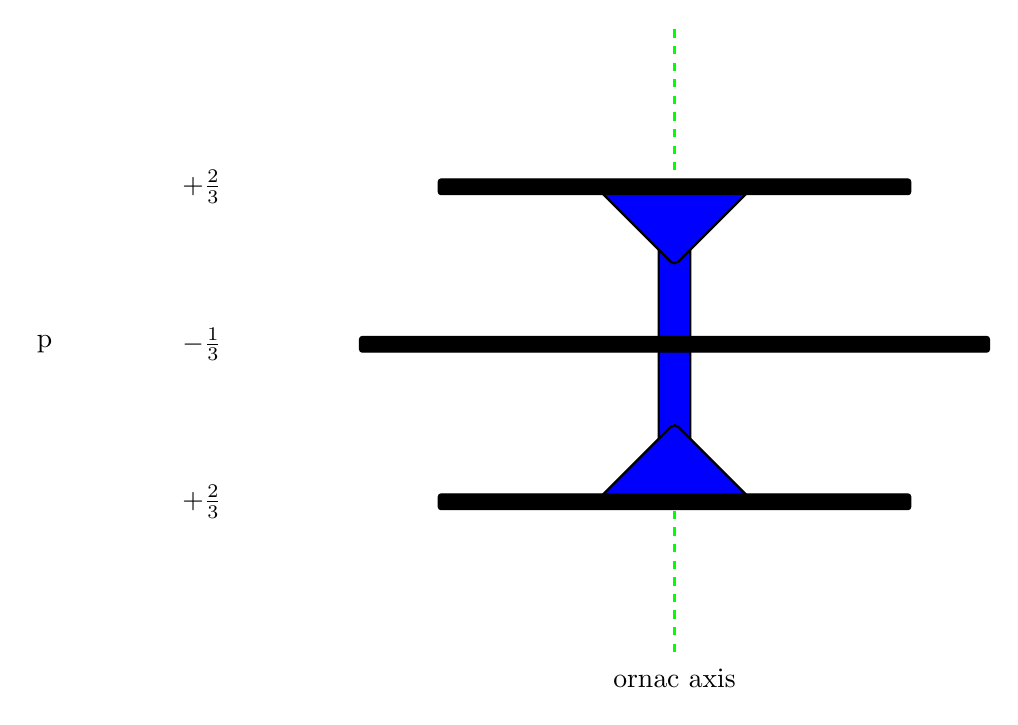
\begin{tikzpicture}[scale=1, rotate=0]


% Ornac axis
\draw[green, dashed, very thick] (4,6) -- (4,-2) ;
\path 
(4,-2) node [below]  {ornac axis};




\path 
(-4,2) node   {p};




% Up quark ornac-pair
\path 
(-2,4) node  (red) {$+\frac{2}{3}$};

% Blue rect to show force
\filldraw[fill=blue, draw=black, thick,rounded corners=2pt] (3.8, 4) rectangle (4.2, 0);

% Blue arrow down
\filldraw[fill=blue, draw=black, thick,rounded corners=2pt] (3,4) -- (5,4) -- (4,3)-- cycle; 

\filldraw[fill=black, draw=black ,rounded corners=1pt] (1, 3.9) rectangle (7, 4.1);


% Down quark ornac-pair
\path 
(-2,2) node  (red) {$-\frac{1}{3}$};

% Red arrow up
%\filldraw[fill=red, draw=black, thick,rounded corners=2pt] (3,2) -- (5,2) -- (4,3)-- cycle; 

% Red arrow down
%\filldraw[fill=red, draw=black, thick,rounded corners=2pt] (3,2) -- (5,2) -- (4,1)-- cycle; 

\filldraw[fill=black, draw=black ,rounded corners=1pt] (0, 1.9) rectangle (8, 2.1);


% Up quark ornac-pair
\path 
(-2,0) node  (red) {$+\frac{2}{3}$};

% Blue arrow up
\filldraw[fill=blue, draw=black, thick,rounded corners=2pt] (3,0) -- (5,0) -- (4,1)-- cycle; 
   

\filldraw[fill=black, draw=black ,rounded corners=1pt] (1,-0.1) rectangle (7, 0.1);





\end{tikzpicture}
\caption{Proton Attractive Force
\label{Fig:Proton_Attractive_Force}}
\end{figure}




\input{./matter_ornac_pairs/Fig:Proton_Repulsice_Force.tex}



%
% Deuteron: quark ornac-pairs with ornac axis
%
\begin{wrapfigure}{r}{0.5\textwidth}
  \begin{center}
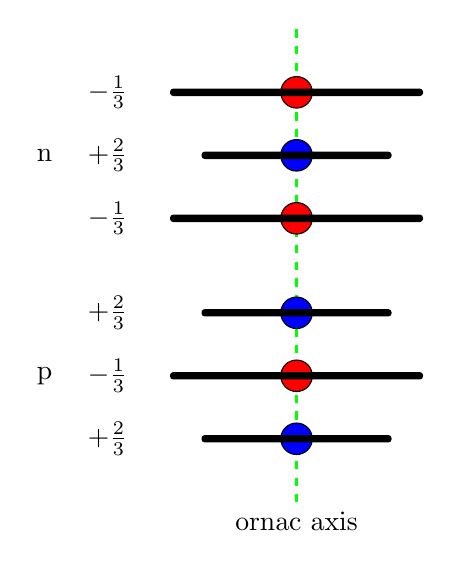
\begin{tikzpicture}[scale=0.4, rotate=0]



% Ornac axis
\draw[green, dashed, very thick] (4,4) -- (4,-11) ;
\path 
(4,-11) node [below]  {ornac axis};

%
% Neutron
%
\path 
(-4,0) node   {n};


% Down quark ornac-pair
\path 
(-2,2) node  (red) {$-\frac{1}{3}$};

\filldraw[fill=red, draw=black] (4,2) circle [radius=0.5];

\filldraw[fill=black, draw=black ,rounded corners=1pt] (0, 1.9) rectangle (8, 2.1);


% Up quark ornac-pair
\path 
(-2,0) node  (red) {$+\frac{2}{3}$};

\filldraw[fill=blue, draw=black] (4,0) circle [radius=0.5];

\filldraw[fill=black, draw=black ,rounded corners=1pt] (1,-0.1) rectangle (7, 0.1);



% Down quark ornac-pair
\path 
(-2,-2) node  (red) {$-\frac{1}{3}$};

\filldraw[fill=red, draw=black] (4,-2) circle [radius=0.5];

\filldraw[fill=black, draw=black ,rounded corners=1pt] (0, -1.9) rectangle (8, -2.1);


%
% Proton
%

\path 
(-4,-7) node   {p};

% Up quark ornac-pair
\path 
(-2,-5) node  (red) {$+\frac{2}{3}$};

\filldraw[fill=blue, draw=black] (4,-5) circle [radius=0.5];

\filldraw[fill=black, draw=black ,rounded corners=1pt] (1, -4.9) rectangle (7, -5.1);



% Down quark ornac-pair
\path 
(-2,-7) node  (red) {$-\frac{1}{3}$};

\filldraw[fill=red, draw=black] (4,-7) circle [radius=0.5];

\filldraw[fill=black, draw=black ,rounded corners=1pt] (0, -6.9) rectangle (8, -7.1);


% Up quark ornac-pair
\path 
(-2, -9) node  (red) {$+\frac{2}{3}$};

\filldraw[fill=blue, draw=black] (4,-9) circle [radius=0.5];

\filldraw[fill=black, draw=black ,rounded corners=1pt] (1,-8.9) rectangle (7, -9.1);



\end{tikzpicture}
\end{center}
\caption{Deuteron from side build up off quark ornac-pairs with ornac axis
\label{fig:Deuteron from side build up off quark ornac-pairs}}
\end{wrapfigure}

% End Deuteron









\begin{figure}
    
    \begin{subfigure}[b]{0.5\textwidth}
        
%
% Proton: quark ornac-pairs
%
%\begin{figure}
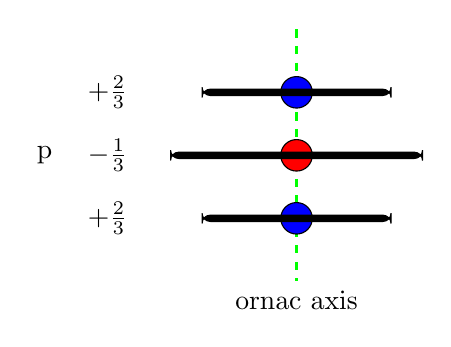
\begin{tikzpicture}[scale=0.4, rotate=0]


% Ornac axis
\draw[green, dashed, very thick] (4,6) -- (4,-2) ;
\path 
(4,-2) node [below]  {ornac axis};




\path 
(-4,2) node   {p};




% Up quark ornac-pair
\path 
(-2,4) node  (red) {$+\frac{2}{3}$};

\filldraw[fill=blue, draw=black] (4,4) circle [radius=0.5];

\filldraw[fill=black, draw=black ,rounded corners=3pt] (1, 3.9) rectangle (7, 4.1);



% Down quark ornac-pair
\path 
(-2,2) node  (red) {$-\frac{1}{3}$};

\filldraw[fill=red, draw=black] (4,2) circle [radius=0.5];

\filldraw[fill=black, draw=black ,rounded corners=3pt] (0, 1.9) rectangle (8, 2.1);


% Up quark ornac-pair
\path 
(-2,0) node  (red) {$+\frac{2}{3}$};

\filldraw[fill=blue, draw=black] (4,0) circle [radius=0.5];

\filldraw[fill=black, draw=black ,rounded corners=3pt] (1,-0.1) rectangle (7, 0.1);





\end{tikzpicture}
\caption{Proton from side build up off quark ornac-pairs 
\label{fig:Proton from side build up off quark ornac-pairs}}
%\end{figure}




    
    \end{subfigure}
    \begin{subfigure}[b]{0.5\textwidth}
        %
% Neutron: quark ornac-pairs
%
%\begin{figure}
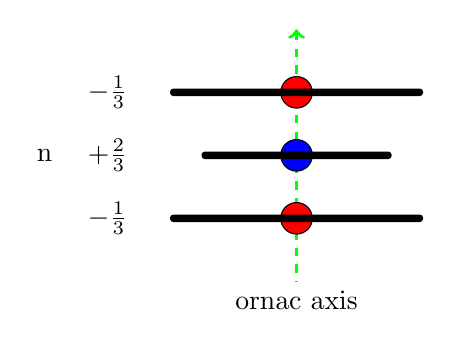
\begin{tikzpicture}[scale=0.4, rotate=0]



% Ornac axis
\draw[green, dashed, very thick, <-] (4,4) -- (4,-4) ;
\path 
(4,-4) node [below]  {ornac axis};




\path 
(-4,0) node   {n};

% Down quark ornac-pair
\path 
(-2,2) node  (red) {$-\frac{1}{3}$};

\filldraw[fill=red, draw=black] (4,2) circle [radius=0.5];

\filldraw[fill=black, draw=black ,rounded corners=1pt] (0, 1.9) rectangle (8, 2.1);


% Up quark ornac-pair
\path 
(-2,0) node  (red) {$+\frac{2}{3}$};

\filldraw[fill=blue, draw=black] (4,0) circle [radius=0.5];

\filldraw[fill=black, draw=black ,rounded corners=1pt] (1,-0.1) rectangle (7, 0.1);



% Down quark ornac-pair
\path 
(-2,-2) node  (red) {$-\frac{1}{3}$};

\filldraw[fill=red, draw=black] (4,-2) circle [radius=0.5];

\filldraw[fill=black, draw=black ,rounded corners=1pt] (0, -1.9) rectangle (8, -2.1);




\end{tikzpicture}
\caption{Neutron from side build up off quark ornac-pairs 
\label{fig:Neutron  from side build up off quark ornac-pairs}}
%\end{figure}




     
    \end{subfigure}

    \caption{Proton next to Neutron}\label{Fig:Proton_next_to_Neutron}
\end{figure}





\begin{figure}
    
    \begin{subfigure}[b]{0.5\textwidth}
        

%
% Helium3: quark ornac-pairs with ornac axis
%
%\begin{figure}
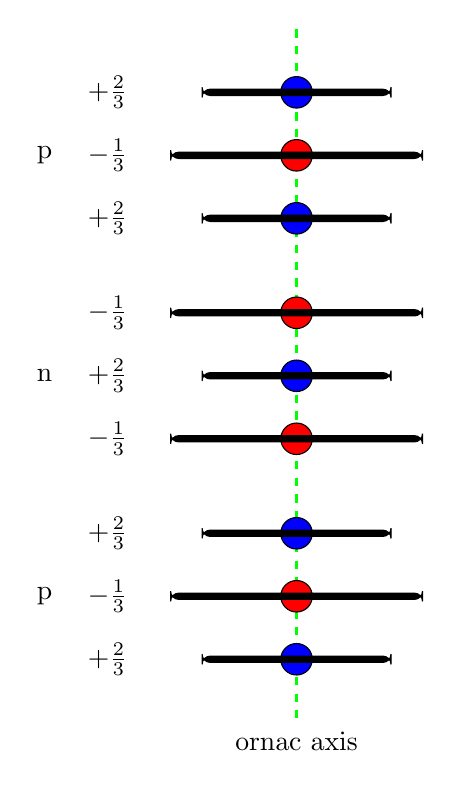
\begin{tikzpicture}[scale=0.4, rotate=0]


% Ornac axis
\draw[green, dashed, very thick] (4,11) -- (4,-11) ;
\path 
(4,-11) node [below]  {ornac axis};

%
% Proton Top
%

\path 
(-4,7) node   {p};

% Up quark ornac-pair
\path 
(-2,9) node  (red) {$+\frac{2}{3}$};

\filldraw[fill=blue, draw=black] (4,9) circle [radius=0.5];

\filldraw[fill=black, draw=black ,rounded corners=3pt] (1, 8.9) rectangle (7, 9.1);



% Down quark ornac-pair
\path 
(-2,7) node  (red) {$-\frac{1}{3}$};

\filldraw[fill=red, draw=black] (4,7) circle [radius=0.5];

\filldraw[fill=black, draw=black ,rounded corners=3pt] (0, 6.9) rectangle (8, 7.1);


% Up quark ornac-pair
\path 
(-2, 5) node  (red) {$+\frac{2}{3}$};

\filldraw[fill=blue, draw=black] (4,5) circle [radius=0.5];

\filldraw[fill=black, draw=black ,rounded corners=3pt] (1,4.9) rectangle (7, 5.1);








%
% Neutron middle
%
\path 
(-4,0) node   {n};


% Down quark ornac-pair
\path 
(-2,2) node  (red) {$-\frac{1}{3}$};

\filldraw[fill=red, draw=black] (4,2) circle [radius=0.5];

\filldraw[fill=black, draw=black ,rounded corners=3pt] (0, 1.9) rectangle (8, 2.1);


% Up quark ornac-pair
\path 
(-2,0) node  (red) {$+\frac{2}{3}$};

\filldraw[fill=blue, draw=black] (4,0) circle [radius=0.5];

\filldraw[fill=black, draw=black ,rounded corners=3pt] (1,-0.1) rectangle (7, 0.1);



% Down quark ornac-pair
\path 
(-2,-2) node  (red) {$-\frac{1}{3}$};

\filldraw[fill=red, draw=black] (4,-2) circle [radius=0.5];

\filldraw[fill=black, draw=black ,rounded corners=3pt] (0, -1.9) rectangle (8, -2.1);


%
% Proton bottom
%

\path 
(-4,-7) node   {p};

% Up quark ornac-pair
\path 
(-2,-5) node  (red) {$+\frac{2}{3}$};

\filldraw[fill=blue, draw=black] (4,-5) circle [radius=0.5];

\filldraw[fill=black, draw=black ,rounded corners=3pt] (1, -4.9) rectangle (7, -5.1);



% Down quark ornac-pair
\path 
(-2,-7) node  (red) {$-\frac{1}{3}$};

\filldraw[fill=red, draw=black] (4,-7) circle [radius=0.5];

\filldraw[fill=black, draw=black ,rounded corners=3pt] (0, -6.9) rectangle (8, -7.1);


% Up quark ornac-pair
\path 
(-2, -9) node  (red) {$+\frac{2}{3}$};

\filldraw[fill=blue, draw=black] (4,-9) circle [radius=0.5];

\filldraw[fill=black, draw=black ,rounded corners=3pt] (1,-8.9) rectangle (7, -9.1);







\end{tikzpicture}
\caption{Helium3 from side build up off quark ornac-pairs with ornac axis
\label{fig:Helium3 from side build up off quark ornac-pairs}}
%\end{figure}

% End Helium3



    
    \end{subfigure}
    \begin{subfigure}[b]{0.5\textwidth}
        

%
% Tritium: quark ornac-pairs with ornac axis
%
%\begin{figure}
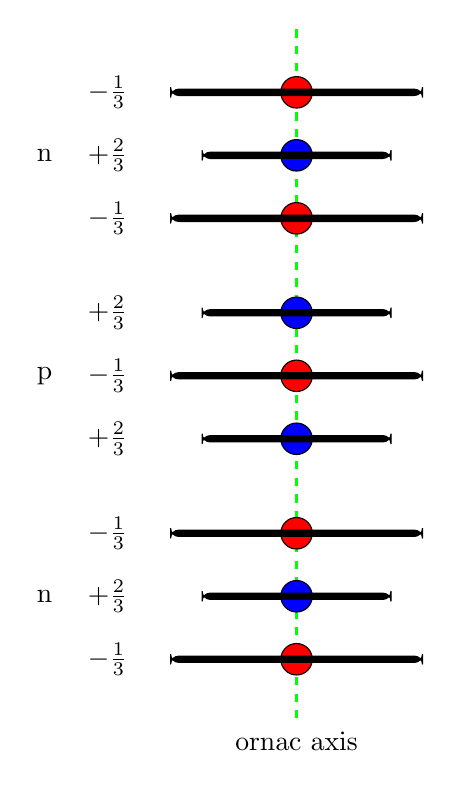
\begin{tikzpicture}[scale=0.4, rotate=0]



% Ornac axis
\draw[green, dashed, very thick] (4,4) -- (4,-18) ;
\path 
(4,-18) node [below]  {ornac axis};

%
% Neutron top
%
\path 
(-4,0) node   {n};


% Down quark ornac-pair
\path 
(-2,2) node  (red) {$-\frac{1}{3}$};

\filldraw[fill=red, draw=black] (4,2) circle [radius=0.5];

\filldraw[fill=black, draw=black ,rounded corners=3pt] (0, 1.9) rectangle (8, 2.1);


% Up quark ornac-pair
\path 
(-2,0) node  (red) {$+\frac{2}{3}$};

\filldraw[fill=blue, draw=black] (4,0) circle [radius=0.5];

\filldraw[fill=black, draw=black ,rounded corners=3pt] (1,-0.1) rectangle (7, 0.1);



% Down quark ornac-pair
\path 
(-2,-2) node  (red) {$-\frac{1}{3}$};

\filldraw[fill=red, draw=black] (4,-2) circle [radius=0.5];

\filldraw[fill=black, draw=black ,rounded corners=3pt] (0, -1.9) rectangle (8, -2.1);


%
% Proton midle
%

\path 
(-4,-7) node   {p};

% Up quark ornac-pair
\path 
(-2,-5) node  (red) {$+\frac{2}{3}$};

\filldraw[fill=blue, draw=black] (4,-5) circle [radius=0.5];

\filldraw[fill=black, draw=black ,rounded corners=3pt] (1, -4.9) rectangle (7, -5.1);



% Down quark ornac-pair
\path 
(-2,-7) node  (red) {$-\frac{1}{3}$};

\filldraw[fill=red, draw=black] (4,-7) circle [radius=0.5];

\filldraw[fill=black, draw=black ,rounded corners=3pt] (0, -6.9) rectangle (8, -7.1);


% Up quark ornac-pair
\path 
(-2, -9) node  (red) {$+\frac{2}{3}$};

\filldraw[fill=blue, draw=black] (4,-9) circle [radius=0.5];

\filldraw[fill=black, draw=black ,rounded corners=3pt] (1,-8.9) rectangle (7, -9.1);



%
% Neutron lower
%
\path 
(-4,-14) node   {n};


% Down quark ornac-pair
\path 
(-2,-12) node  (red) {$-\frac{1}{3}$};

\filldraw[fill=red, draw=black] (4,-12) circle [radius=0.5];

\filldraw[fill=black, draw=black ,rounded corners=3pt] (0, -11.9) rectangle (8, -12.1);


% Up quark ornac-pair
\path 
(-2,-14) node  (red) {$+\frac{2}{3}$};

\filldraw[fill=blue, draw=black] (4,-14) circle [radius=0.5];

\filldraw[fill=black, draw=black ,rounded corners=3pt] (1,-13.9) rectangle (7, -14.1);



% Down quark ornac-pair
\path 
(-2,-16) node  (red) {$-\frac{1}{3}$};

\filldraw[fill=red, draw=black] (4,-16) circle [radius=0.5];

\filldraw[fill=black, draw=black ,rounded corners=3pt] (0, -15.9) rectangle (8, -16.1);




\end{tikzpicture}
\caption{Tritium from side build up off quark ornac-pairs with ornac axis
\label{fig:Tritium from side build up off quark ornac-pairs}}
%\end{figure}

% End Tritium





     
    \end{subfigure}

    \caption{Helium3 next to Tritium}\label{fig:Helium3_next_to_Tritium}
\end{figure}

%%
% Neutron: quark ornac-pairs with ornac axis
%
\begin{figure}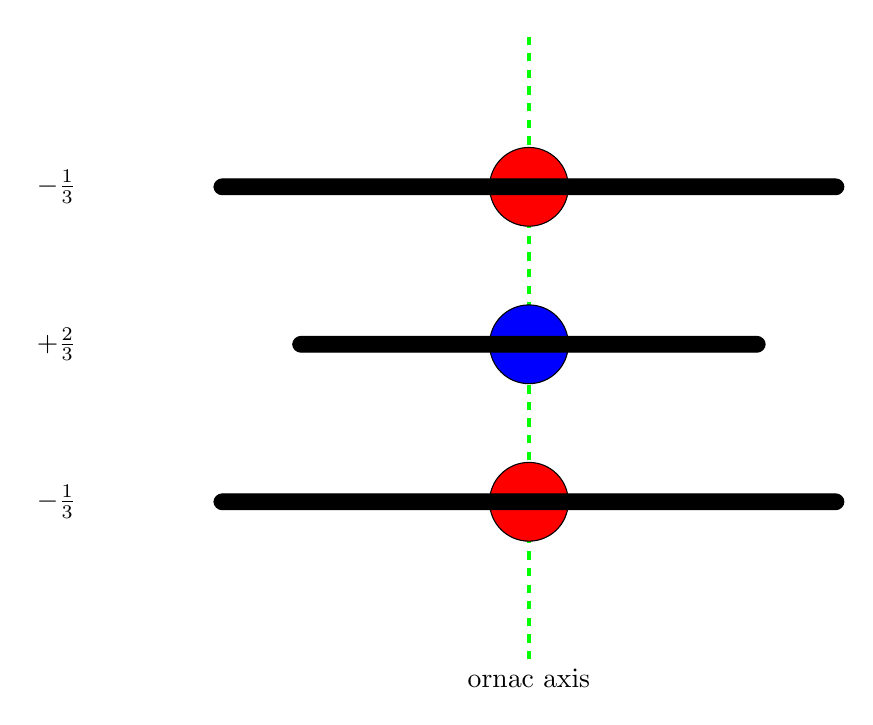
\begin{tikzpicture}[scale=1, rotate=0]



% Ornac axis
\draw[green, dashed, very thick] (4,-4) -- (4,4) ;
\path 
(4,-4) node [below]  {ornac axis};


% Down quark ornac-pair
\path 
(-2,2) node  (red) {$-\frac{1}{3}$}
(4, 2) node[circle,draw, fill=blue] (red) {};

\filldraw[fill=red, draw=black] (4,2) circle [radius=0.5];

\filldraw[fill=black, draw=black ,rounded corners=3pt] (0, 1.9) rectangle (8, 2.1);


% Up quark ornac-pair
\path 
(-2,0) node  (red) {$+\frac{2}{3}$}
(4, 0) node[circle,draw, fill=blue] (blue) {};

\filldraw[fill=blue, draw=black] (4,0) circle [radius=0.5];

\filldraw[fill=black, draw=black ,rounded corners=3pt] (1,-0.1) rectangle (7, 0.1);



% Down quark ornac-pair
\path 
(-2,-2) node  (red) {$-\frac{1}{3}$}
(4, -2) node[circle,draw, fill=blue] (red) {};

\filldraw[fill=red, draw=black] (4,-2) circle [radius=0.5];

\filldraw[fill=black, draw=black ,rounded corners=3pt] (0, -1.9) rectangle (8, -2.1);





\end{tikzpicture}
\caption{Neutron from side build up off quark ornac-pairs with ornac axis
\label{fig:Neutron  from side build up off quark ornac-pairs}}
\end{figure}






%
% Neutron: quark ornac-pairs
%
\begin{figure}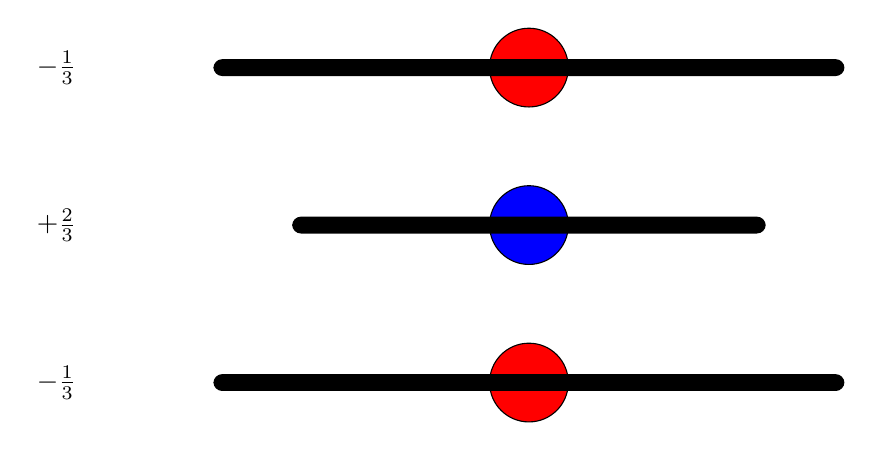
\begin{tikzpicture}[scale=1, rotate=0]




% Down quark ornac-pair
\path 
(-2,2) node  (red) {$-\frac{1}{3}$}
(4, 2) node[circle,draw, fill=blue] (red) {};

\filldraw[fill=red, draw=black] (4,2) circle [radius=0.5];

\filldraw[fill=black, draw=black ,rounded corners=3pt] (0, 1.9) rectangle (8, 2.1);


% Up quark ornac-pair
\path 
(-2,0) node  (red) {$+\frac{2}{3}$}
(4, 0) node[circle,draw, fill=blue] (blue) {};

\filldraw[fill=blue, draw=black] (4,0) circle [radius=0.5];

\filldraw[fill=black, draw=black ,rounded corners=3pt] (1,-0.1) rectangle (7, 0.1);



% Down quark ornac-pair
\path 
(-2,-2) node  (red) {$-\frac{1}{3}$}
(4, -2) node[circle,draw, fill=blue] (red) {};

\filldraw[fill=red, draw=black] (4,-2) circle [radius=0.5];

\filldraw[fill=black, draw=black ,rounded corners=3pt] (0, -1.9) rectangle (8, -2.1);




\end{tikzpicture}
\caption{Neutron from side build up off quark ornac-pairs 
\label{fig:Neutron  from side build up off quark ornac-pairs}}
\end{figure}





%
% Proton: quark ornac-pairs
%
\begin{figure}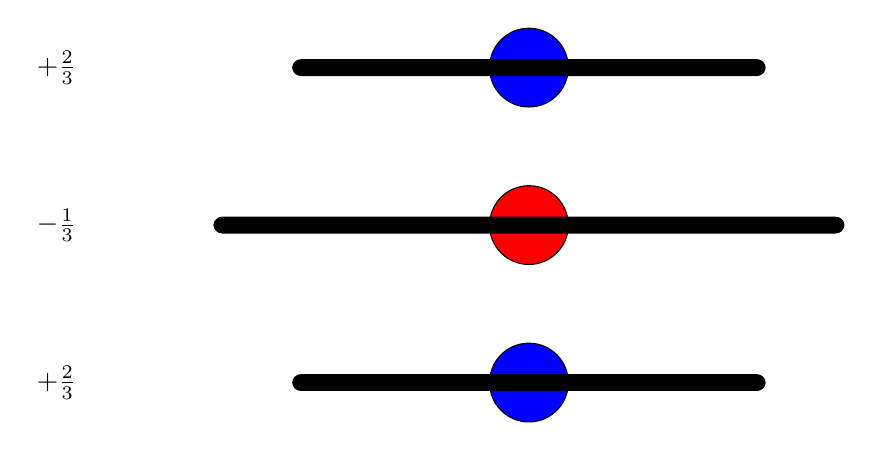
\begin{tikzpicture}[scale=1, rotate=0]

% Up quark ornac-pair
\path 
(-2,4) node  (red) {$+\frac{2}{3}$}
(4, 4) node[circle,draw, fill=blue] (blue) {};

\filldraw[fill=blue, draw=black] (4,4) circle [radius=0.5];

\filldraw[fill=black, draw=black ,rounded corners=3pt] (1, 3.9) rectangle (7, 4.1);



% Down quark ornac-pair
\path 
(-2,2) node  (red) {$-\frac{1}{3}$}
(4, 2) node[circle,draw, fill=blue] (red) {};

\filldraw[fill=red, draw=black] (4,2) circle [radius=0.5];

\filldraw[fill=black, draw=black ,rounded corners=3pt] (0, 1.9) rectangle (8, 2.1);


% Up quark ornac-pair
\path 
(-2,0) node  (red) {$+\frac{2}{3}$}
(4, 0) node[circle,draw, fill=blue] (blue) {};

\filldraw[fill=blue, draw=black] (4,0) circle [radius=0.5];

\filldraw[fill=black, draw=black ,rounded corners=3pt] (1,-0.1) rectangle (7, 0.1);





\end{tikzpicture}
\caption{Proton from side build up off quark ornac-pairs 
\label{fig:Proton from side build up off quark ornac-pairs}}
\end{figure}




%
% Up quark ornac-pair solo
%
\begin{figure}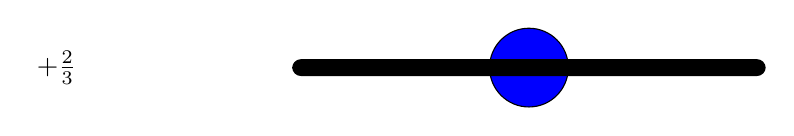
\begin{tikzpicture}[scale=1, rotate=0]


\path 
(-2,0) node  (red) {$+\frac{2}{3}$}
(4, 0) node[circle,draw, fill=blue] (blue) {};

\filldraw[fill=blue, draw=black] (4,0) circle [radius=0.5];

\filldraw[fill=black, draw=black ,rounded corners=3pt] (1,-0.1) rectangle (7, 0.1);


\end{tikzpicture}
\caption{Up quark ornac-pair from side
\label{fig:Up quark ornac-pair from side}}
\end{figure}












\section{Photon vertical with speed vectors}
\begin{figure}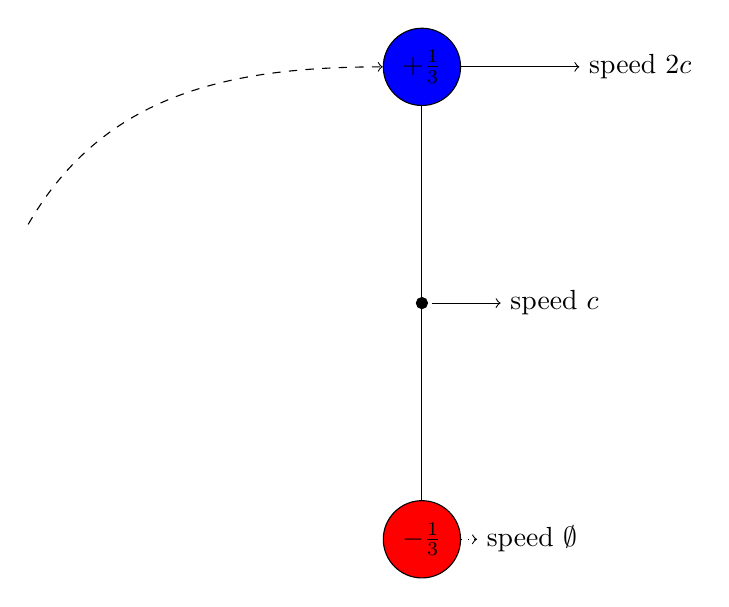
\begin{tikzpicture}[scale=1, rotate=0]

% photon vertical with speed vectors

\path 
(0,0) node[circle,draw, fill=red]  (red) {$-\frac{1}{3}$}
(0,6) node[circle,draw, fill=blue] (blue) {$+\frac{1}{3}$};
\draw[black] (red) -- (blue)         node[pos=0.5](center){};
\filldraw
 (center) circle (2pt);
\draw[->, black] (center) -- ++(1,0) node [anchor=west]{speed $c$};
\draw[->, black] (blue) -- ++(2,0) node [anchor=west]{speed $2c$};
\draw[->, dotted] (red) -- ++(0.7,0) node [anchor=west]{speed $\emptyset$};

\draw[->,dashed] (-5,4) to[out=60,in=180] (blue);

\end{tikzpicture}
\caption{Photon vertical with speed vectors 
\label{fig:photon_vertical}}
\end{figure}


\section{Quark ornac-pair vertical with green and yellow area for \\
 sub and hyper c  indication speed}
\begin{figure}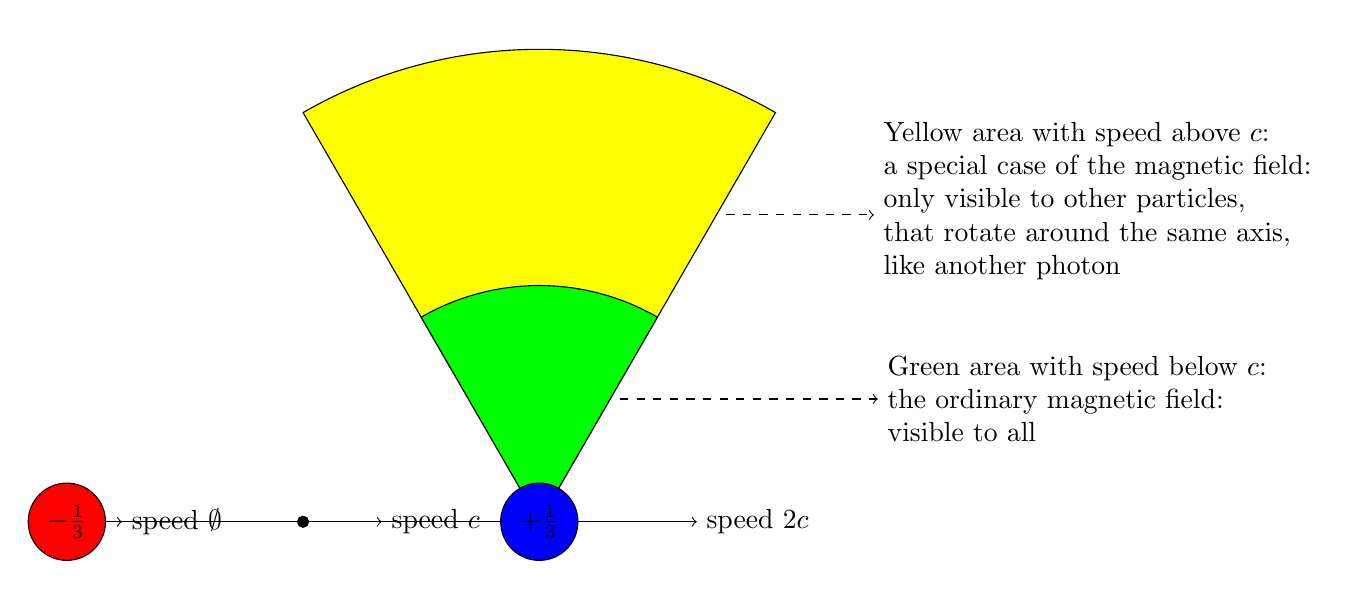
\begin{tikzpicture}[scale=1, rotate=0]

% Quark ornac-pair vertical with green and yellow area for 
% sub and hyper c  indication speed 

\filldraw[fill=yellow, draw=black] (0,0) -- (60:6) 
node[pos=0.75, ](yellow) {} 
arc (60:120:6) -- (0,0);
\draw[->, dashed, black] (yellow) -- ++(2,0) node [right, align=left]
{Yellow area with speed above $c$: \\ 
a special case of the magnetic field: \\
only visible to other particles,  \\ 
that rotate around the same axis, \\
like another photon \\
};

\filldraw[fill=green, draw=black] (0,0) -- (60:3) 
node[pos=0.6, ](green) {} 
arc (60:120:3) -- (0,0);
\draw[->, dashed, black] (green) -- ++(3.4,0) node [right , align=left]
{
Green area with speed below $c$: \\ 
the ordinary magnetic field: \\ 
visible to all};


\path 
(-6,0) node[circle,draw, fill=red]  (red) {$-\frac{1}{3}$}
(0,0) node[circle,draw, fill=blue] (blue) {$+\frac{1}{3}$};
\draw[black] (red) -- (blue)         node[pos=0.5](center){};
\filldraw
 (center) circle (2pt);
\draw[->, black] (center) -- ++(1,0) node [anchor=west]{speed $c$};
\draw[->, black] (blue) -- ++(2,0) node [anchor=west]{speed $2c$};
\draw[->, dotted] (red) -- ++(0.7,0) node [anchor=west]{speed $\emptyset$};

%\draw[->,dashed] (-5,4) to[out=60,in=180] (blue);



\end{tikzpicture}\caption{Down quark ornac-pair  with green and yellow area for \\
 sub and hyper c  indication speed 
\label{fig:down_quark_green_yellow}}
\end{figure}



\section{Photon horizontal with speed vectors}
\begin{figure}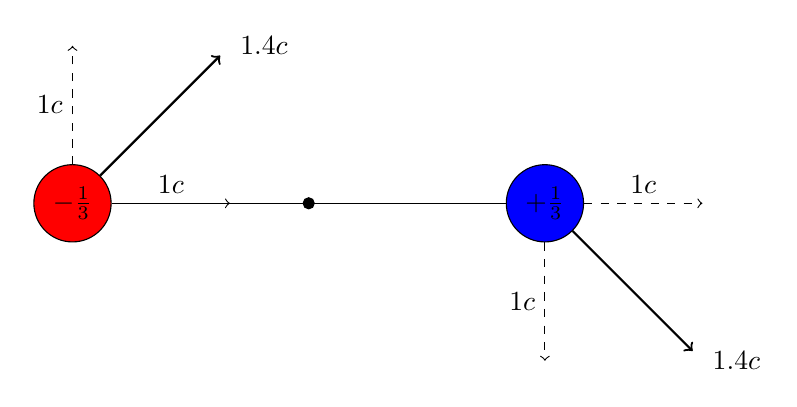
\begin{tikzpicture}[scale=1, rotate=0]


% photon horizontal with speed vectors



\path 
(0,0) node[circle,draw, fill=red](red) {$-\frac{1}{3}$}
(6,0) node[circle,draw, fill=blue](blue) {$+\frac{1}{3}$};
\draw[black] (red) -- (blue)          node[pos=0.5](center){};
\filldraw
 (center) circle (2pt);
%\draw[->, black] (center) -- ++(1,0) node [anchor=west]{};

%% Arrows indicating the speed components from blue
\draw[->, black, dashed] (blue) -- node[above] { $1c$} ++(2,0) node [](west){};
\draw[->, black, dashed] (blue) -- node[left] { $1c$} ++(0,-2) node [](south){};
\path (west) -- ++(0,-2) node [](southwest){};
%\draw[ black, dotted] (west) -- ++(0,-2) node [](southwest){};
%\draw[ black, dotted] (south) -- (southwest) node []{};
\draw[->, black, thick] (blue) --  (southwest) node[below, right] { $1.4c$};

%% Arrows indicating the speed components from red
\draw[->, black, dashed] (red) -- node[above] { $1c$} ++(2,0) node [](redwest){};
\draw[->, black, dashed] (red) -- node[left] { $1c$} ++(0,2) node [](redsouth){};
\path(redwest) -- ++(0,2) node [](redsouthwest){};
%\draw[ black, dotted] (redwest) -- ++(0,1.5) node []{};
%\draw[ black, dotted] (redsouth) -- ++(1.5,0) node []{};
\draw[->, black, thick] (red) --  (redsouthwest) node[below, right] { $1.4c$};




\end{tikzpicture}\caption{Photon horizontal with speed vectors
\label{fig:photon_horizontal}}
\end{figure}

\section{Photon diagonal with speed vectors}

\begin{figure}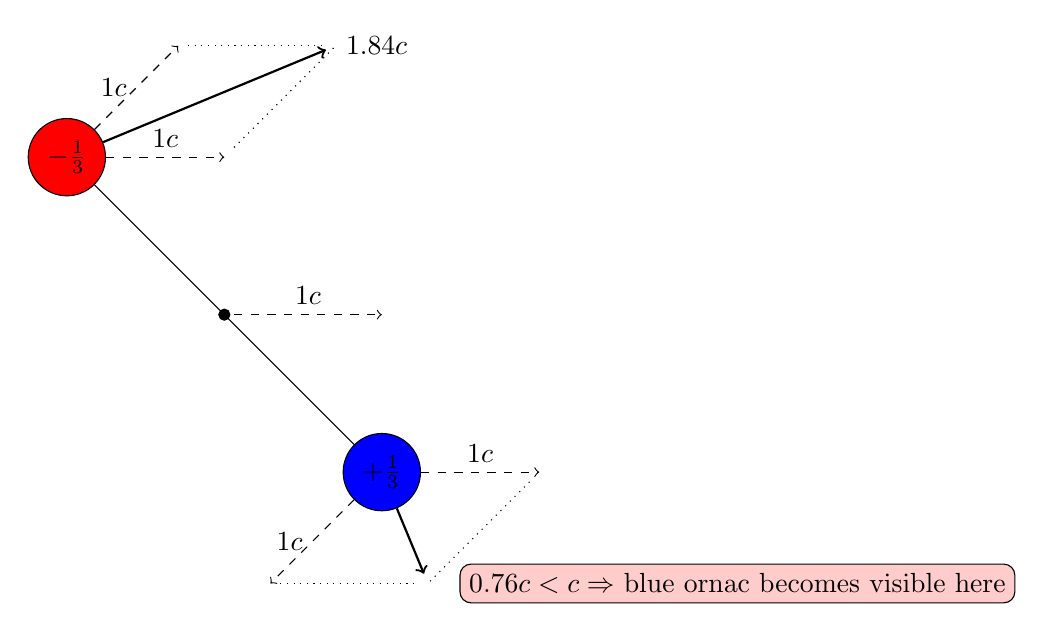
\begin{tikzpicture}[scale=1, rotate=0]


% photon diagonal with speed vectors



\path 
(0,4) node[circle,draw, fill=red](red) {$-\frac{1}{3}$}
(4,0) node[circle,draw, fill=blue](blue) {$+\frac{1}{3}$};
\draw[black] (red) -- (blue)          node[pos=0.5](center){};
\filldraw
 (center) circle (2pt);
\draw[->,dashed, black] (center) -- node[above] { $1c$} ++(2,0) node [anchor=west]{};

%% Arrows indicating the speed components from blue
\draw[->, black, dashed] (blue) -- node[above] { $1c$} ++(2,0) node [](west){};
\draw[->, black, dashed] (blue) -- node[left] { $1c$} ++(225:2) node [](south){};
\draw[ black, dotted] (west) -- ++(225:2) node [](southwest){};
\draw[ black, dotted] (south) -- (southwest) node []{};
\draw[->, black, thick] (blue) --  (southwest) node (under_c) {};
\path
(under_c)+(0.4,0)node [fill=red!20,draw, rounded corners, right]
{ $0.76c < c \Rightarrow$ blue ornac becomes visible here};

%% Arrows indicating the speed components from red
\draw[->, black, dashed] (red) -- node[above] { $1c$} ++(2,0) node [](redwest){};
\draw[->, black, dashed] (red) -- node[left] { $1c$} ++(45:2) node [](redsouth){};
\draw[ black, dotted] (redwest) -- ++(45:2) node [](redsouthwest){};
\draw[ black, dotted] (redsouth) -- (redsouthwest) node []{};
\draw[->, black, thick] (red) --  (redsouthwest) node [below, right] { $1.84c$};

\end{tikzpicture}\caption{Photon diagonal with speed vectors\label{fig:photon-diagonal}}
\end{figure}


\section{Photon going through cycloid cycle in colors}
\begin{figure}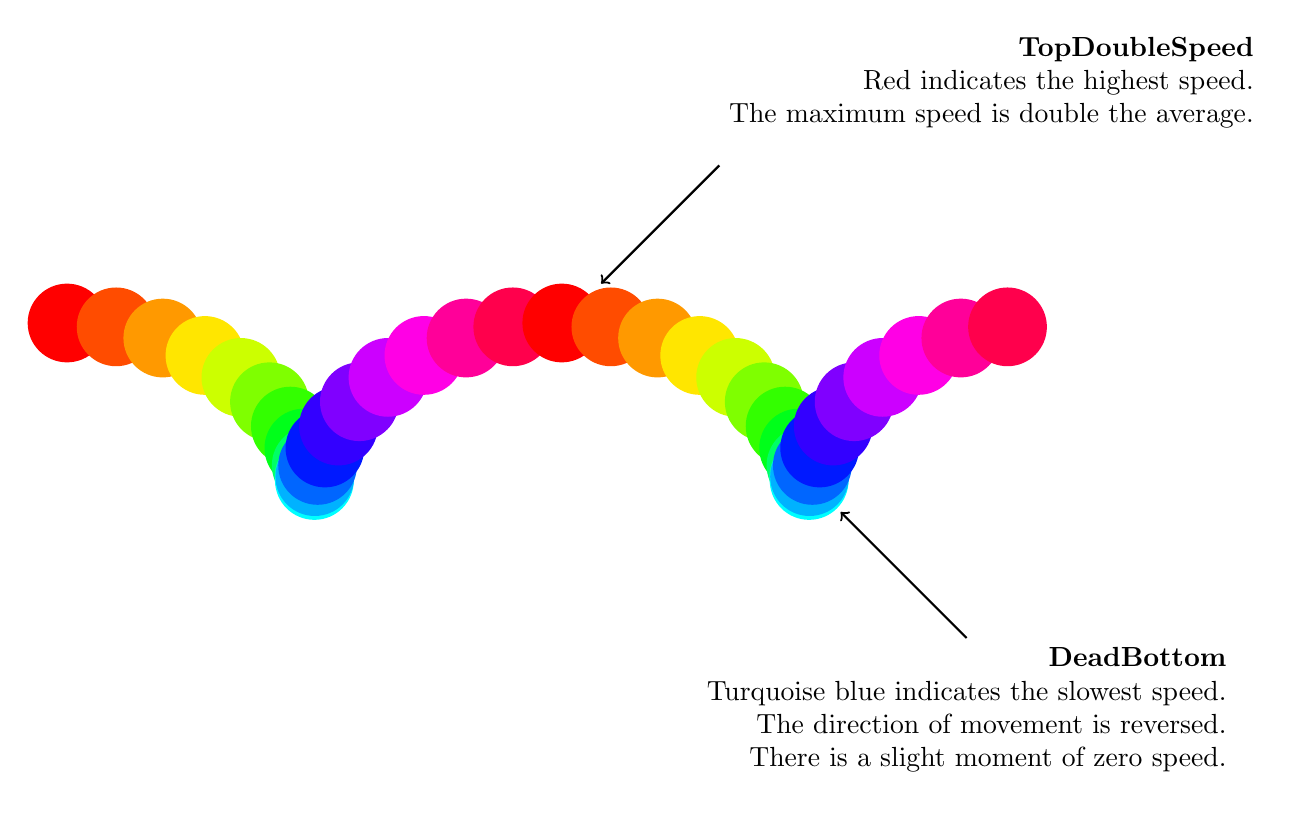
\begin{tikzpicture}[scale=1, rotate=0]

% photon going through cycloid cycle in colors
 \foreach \x in {0, 0.05,...,1}
  {
  \definecolor{reddish}{hsb}{\x, 1, 1}
  \draw[draw=none, fill=reddish] 
   ({((2*pi*\x + sin(2*pi*\x r)) },{1 + cos(2*pi*\x r) }) circle [radius=0.5];

  }

 \foreach \x in {0, 0.05,...,1}
  {
  \definecolor{reddish}{hsb}{\x, 1, 1}
  \draw[draw=none, fill=reddish] 
   ({((2*pi + 2*pi*\x + sin(2*pi*\x r)) },{1 + cos(2*pi*\x r) }) circle [radius=0.5];
  }

\path
(2*pi,2) node (topdoublespeed) {}
(3*pi,0) node (deadbottom2) {};
\draw[<-, thick] (topdoublespeed) +(0.5, 0.5) -- ++(2,2) node (topdoublespeedtext){}; 
\draw[<-, thick] (deadbottom2)+(0.4,-0.4) -- ++(2,-2) node (deadbottomtext) {}; 
\path
(topdoublespeedtext) node [anchor=south west,  align=right]
{\textbf{TopDoubleSpeed} \\
Red indicates the highest speed.\\
The maximum speed is double the average. \\
};
\path
(deadbottomtext) node [below , align=right]
{\textbf{DeadBottom} \\
Turquoise blue indicates the slowest speed.\\
The direction of movement is reversed. \\  
There is a slight moment of zero speed. \\
};


\end{tikzpicture}\caption{Photon going through cycloid cycle in colors
\label{fig:photon_cycloid_colors}}
\end{figure}



\section{Cycloid cycle in colors single ornac of a photon \\ with wheel}
\begin{figure}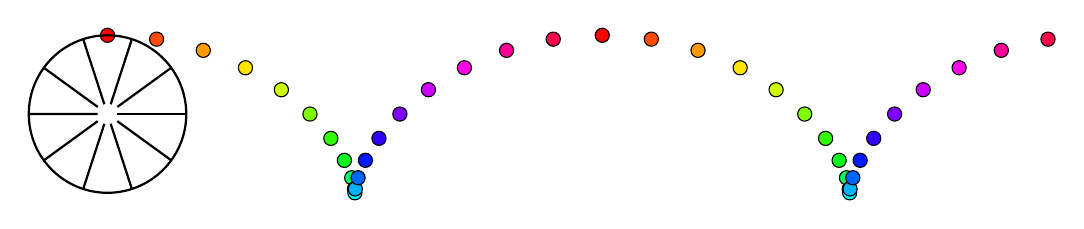
\begin{tikzpicture}[scale=1, rotate=0]

% single ornac of a photon going through cycloid cycle in colors

 \foreach \x in {0, 0.05,...,1}
  {
  \definecolor{reddish}{hsb}{\x, 1, 1}
  \draw[black, fill=reddish] 
   ({((2*pi*\x + sin(2*pi*\x r)) },{1 + cos(2*pi*\x r) }) circle [radius=0.09];
  }
% second cycle
 \foreach \x in {0, 0.05,...,1}
  {
  \definecolor{reddish}{hsb}{\x, 1, 1}
  \draw[black, fill=reddish] 
   ({((2*pi + 2*pi*\x + sin(2*pi*\x r)) },{1 + cos(2*pi*\x r) }) circle [radius=0.09];
  }


% wheel
\path
(0,1) node (hub) {};
\draw[black, thick]
(hub) circle[radius=1];
% arrow

%\draw[->, thick]
%(hub)++(215:1.5) arc  (315:225:1.5);
% spokes
 \foreach \phi in {0, 0.1,...,1}
  {
%  \definecolor{reddish}{hsb}{\x, 1, 1}
  \draw[black, thick] 
   (hub)-- ++(360*\phi :1);
  }

\end{tikzpicture}\caption{Cycloid cycle in colors single ornac of a photon with wheel
\label{fig:cycloid_wheel}}
\end{figure}



\section{Single ornac of a photon  going through two cycloid cycle in red}
\begin{figure}\begin{tikzpicture}[scale=1, rotate=0]

% single ornac of a photon  going through two cycloid cycle in red

%% red ornac
 \foreach \x in {0, 0.05,...,2}
  {
  
  \draw[black, fill=red] 
   ({((2*pi*\x + sin(2*pi*\x r)) },{1 + cos(2*pi*\x r) }) circle [radius=0.05];

  }

\path
(3*pi,0) node (bottom){};

\draw[<-, thick] (bottom) -- ++(1,-1) node (slowspeed){}; 
\path
(slowspeed) node [anchor=west, align=right]{Slowest speed = $\emptyset$.};

\end{tikzpicture}\caption{Single ornac of a photon  going through two cycloid cycle in red
\label{fig:photon_red_ornac}}
\end{figure}




\section{Single ornac of a photon  going through two cycloid cycle in red
 with green oval to indicate the under c area}
\begin{figure}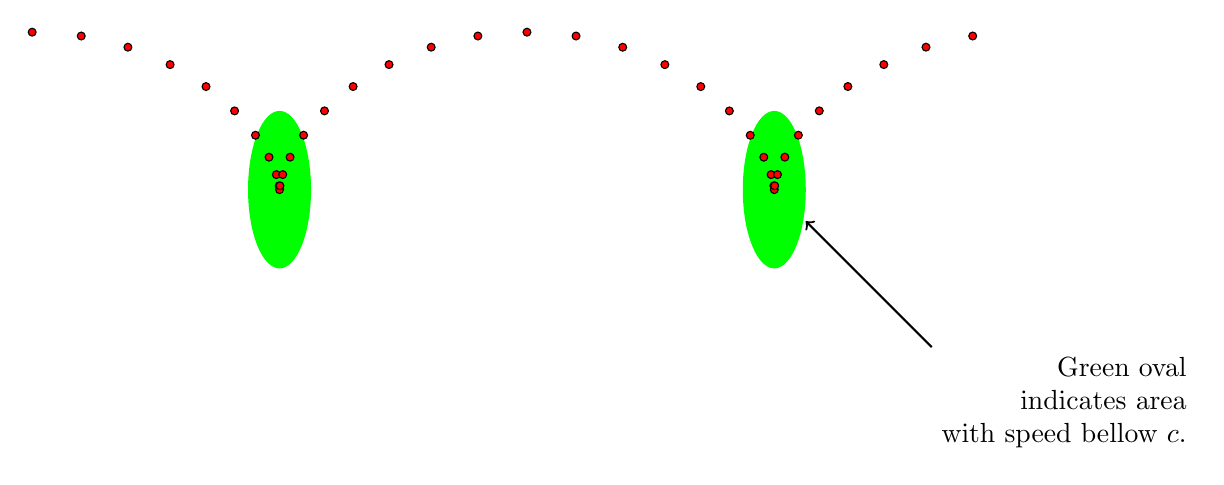
\begin{tikzpicture}[scale=1, rotate=0]

% single ornac of a photon  going through two cycloid cycle in red
% with green oval to indicate the under c area

% greeen oval
\path
(pi,0) node (bottom1){}
(3*pi,0) node (bottom2){};
\draw [draw = none, fill = green]
 (bottom1) circle [ x radius = 0.4, y radius = 1 ]
 (bottom2) circle [ x radius = 0.4, y radius = 1 ]node (greenoval) {};

\draw[<-, thick] (greenoval)+(0.4,-0.4) -- ++(2,-2) node (slowspeed){}; 
\path
(slowspeed) node [below right , align=right]
{Green oval \\ indicates area \\ with  speed bellow $c$.};


%% red ornac
 \foreach \x in {0, 0.05,...,2}
  {
    \draw[black, fill=red] 
   ({((2*pi*\x + sin(2*pi*\x r)) },{1 + cos(2*pi*\x r) }) circle [radius=0.05];
  }


\end{tikzpicture}\caption{Single ornac of a photon  going through two cycloid cycle in red
 with green oval to indicate the under c area
\label{fig:photon_red_ornac_green_area}}
\end{figure}



\section{Two ornac of a photon  going through two cycloid cycle in red and blue}
\begin{figure}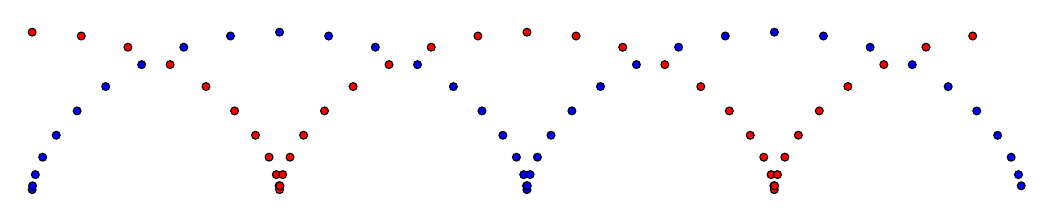
\begin{tikzpicture}[scale=1, rotate=0]

% two ornac of a photon  going through two cycloid cycle in red

%% red ornac
 \foreach \x in {0, 0.05,...,2}
  {
    \draw[black, fill=red] 
   ({((2*pi*\x + sin(2*pi*\x r)) },{1 + cos(2*pi*\x r) }) circle [radius=0.05];
  }


%% blue ornac
 \foreach \x in {0, 0.05,...,2}
  {
    \draw[black, fill=blue] 
   ({((2*pi*\x + sin((2*pi*\x -pi) r)) },{1 + cos((2*pi*\x -pi) r) }) circle [radius=0.05];
  }

\end{tikzpicture}
\caption{Two ornac of a photon  going through two cycloid cycle in red and blue
\label{fig:two_ornac_cycloid}}
\end{figure}


\section{Two ornac of a photon  going through two cycloid cycle in red and blue
 with green oval to indicate the under c area}
\begin{figure}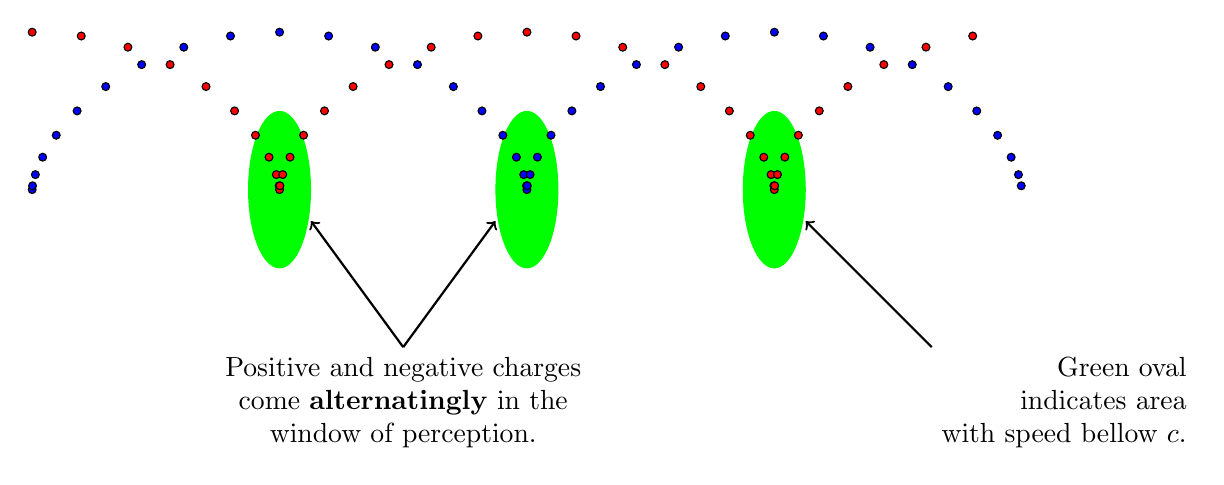
\begin{tikzpicture}[scale=1, rotate=0]

% two ornac of a photon  going through two cycloid cycle in red and blue
% with green oval to indicate the under c area

% greeen ovals
 \foreach \p in {1,...,3}
    \draw [draw = none, fill = green]
     (pi*\p,0) circle [ x radius = 0.4, y radius = 1 ];

\path
(3*pi,0) node (greenoval) {};
\draw[<-, thick] (greenoval)+(0.4,-0.4) -- ++(2,-2) node (slowspeed){}; 
\path
(slowspeed) node [below right , align=right]
{Green oval \\ indicates area \\ with  speed bellow $c$.};

\path
(1*pi,0) node (greenoval1) {}
(2*pi,0) node (greenoval2) {};
\draw[<-, thick] (greenoval1)+(0.4,-0.4) -- (1.5*pi,-2) node (alternatingly){}; 
\draw[<-, thick] (greenoval2)+(-0.4,-0.4) -- (1.5*pi,-2) node {}; 
\path
(alternatingly) node [below , align=center]
{Positive and negative charges \\ 
come  \textbf{alternatingly} in the \\ 
window of perception.};


%% red ornac
 \foreach \x in {0, 0.05,...,2}
  {
    \draw[black, fill=red] 
   ({((2*pi*\x + sin(2*pi*\x r)) },{1 + cos(2*pi*\x r) }) circle [radius=0.05];
  }


%% blue ornac
 \foreach \x in {0, 0.05,...,2}
  {
    \draw[black, fill=blue] 
   ({((2*pi*\x + sin((2*pi*\x -pi) r)) },{1 + cos((2*pi*\x -pi) r) }) circle [radius=0.05];
  }

\end{tikzpicture}\caption{Two ornac of a photon  going through two cycloid cycle in red and blue
 with green oval to indicate the under c area
\label{fig:two_ornac_cycloid_green_area}}
\end{figure}



%
\section{}
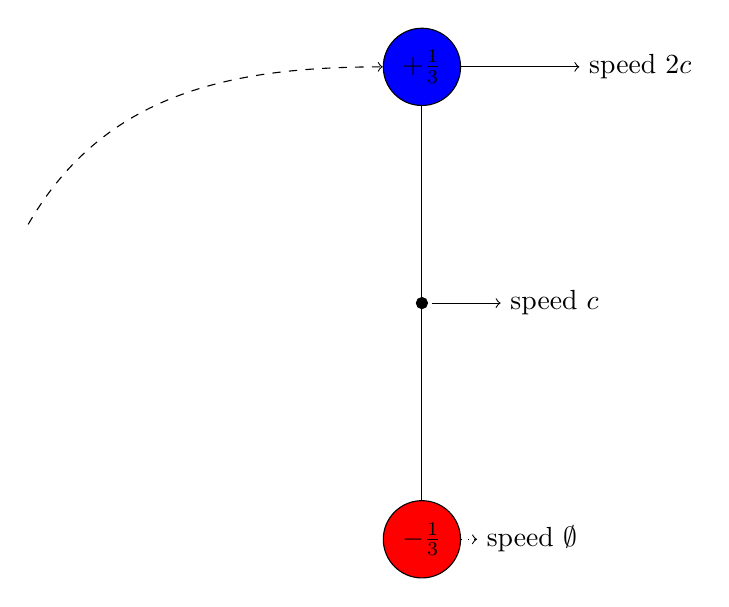
\begin{tikzpicture}[scale=1, rotate=0]

% photon vertical with speed vectors

\path 
(0,0) node[circle,draw, fill=red]  (red) {$-\frac{1}{3}$}
(0,6) node[circle,draw, fill=blue] (blue) {$+\frac{1}{3}$};
\draw[black] (red) -- (blue)         node[pos=0.5](center){};
\filldraw
 (center) circle (2pt);
\draw[->, black] (center) -- ++(1,0) node [anchor=west]{speed $c$};
\draw[->, black] (blue) -- ++(2,0) node [anchor=west]{speed $2c$};
\draw[->, dotted] (red) -- ++(0.7,0) node [anchor=west]{speed $\emptyset$};

\draw[->,dashed] (-5,4) to[out=60,in=180] (blue);

\end{tikzpicture}


\section{}
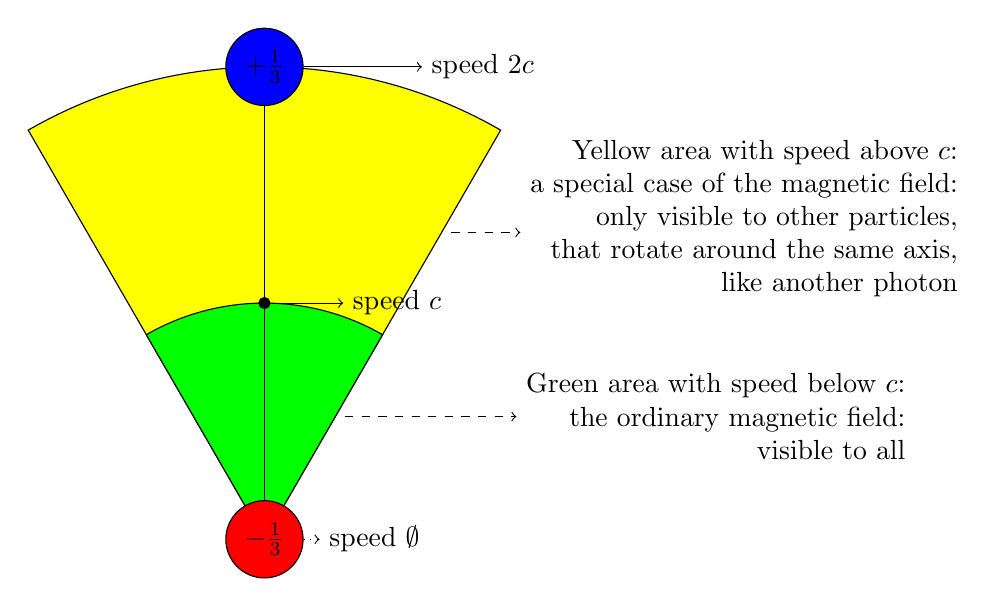
\begin{tikzpicture}[scale=1, rotate=0]

% photon vertical with green and yellow area for 
% sub and hyper c  indication speed vectors

\filldraw[fill=yellow, draw=black] (0,0) -- (60:6) 
node[pos=0.75, ](yellow) {} 
arc (60:120:6) -- (0,0);
\draw[->, dashed, black] (yellow) -- ++(1,0) node [right, align=right]
{Yellow area with speed above $c$: \\ 
a special case of the magnetic field: \\
only visible to other particles,  \\ 
that rotate around the same axis, \\
like another photon \\
};

\filldraw[fill=green, draw=black] (0,0) -- (60:3) 
node[pos=0.6, ](green) {} 
arc (60:120:3) -- (0,0);
\draw[->, dashed, black] (green) -- ++(2.3,0) node [right , align=right]
{
Green area with speed below $c$: \\ 
the ordinary magnetic field: \\ 
visible to all};


\path 
(0,0) node[circle,draw, fill=red]  (red) {$-\frac{1}{3}$}
(0,6) node[circle,draw, fill=blue] (blue) {$+\frac{1}{3}$};
\draw[black] (red) -- (blue)         node[pos=0.5](center){};
\filldraw
 (center) circle (2pt);
\draw[->, black] (center) -- ++(1,0) node [anchor=west]{speed $c$};
\draw[->, black] (blue) -- ++(2,0) node [anchor=west]{speed $2c$};
\draw[->, dotted] (red) -- ++(0.7,0) node [anchor=west]{speed $\emptyset$};

%\draw[->,dashed] (-5,4) to[out=60,in=180] (blue);



\end{tikzpicture}



\section{}
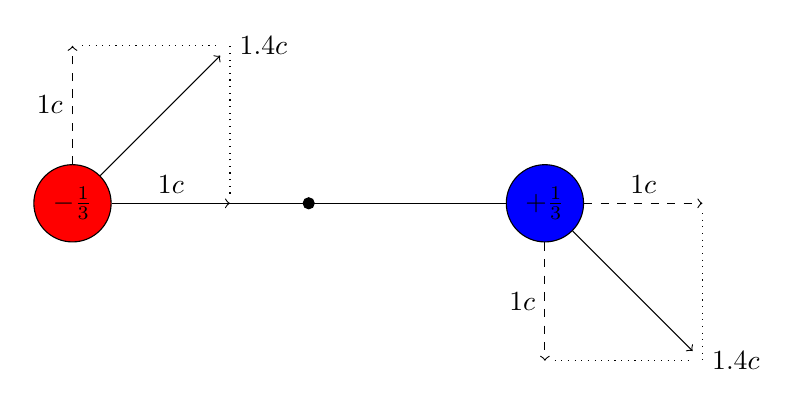
\begin{tikzpicture}[scale=1, rotate=0]


% photon horizontal with speed vectors



\path 
(0,0) node[circle,draw, fill=red](red) {$-\frac{1}{3}$}
(6,0) node[circle,draw, fill=blue](blue) {$+\frac{1}{3}$};
\draw[black] (red) -- (blue)          node[pos=0.5](center){};
\filldraw
 (center) circle (2pt);
%\draw[->, black] (center) -- ++(1,0) node [anchor=west]{};

%% Arrows indicating the speed components from blue
\draw[->, black, dashed] (blue) -- node[above] { $1c$} ++(2,0) node [](west){};
\draw[->, black, dashed] (blue) -- node[left] { $1c$} ++(0,-2) node [](south){};
\draw[ black, dotted] (west) -- ++(0,-2) node [](southwest){};
\draw[ black, dotted] (south) -- (southwest) node []{};
\draw[->, black] (blue) --  (southwest) node[below, right] { $1.4c$};

%% Arrows indicating the speed components from red
\draw[->, black, dashed] (red) -- node[above] { $1c$} ++(2,0) node [](redwest){};
\draw[->, black, dashed] (red) -- node[left] { $1c$} ++(0,2) node [](redsouth){};
\draw[ black, dotted] (redwest) -- ++(0,2) node [](redsouthwest){};
\draw[ black, dotted] (redsouth) -- (redsouthwest) node []{};
\draw[->, black] (red) --  (redsouthwest) node[below, right] { $1.4c$};




\end{tikzpicture}

\section{}

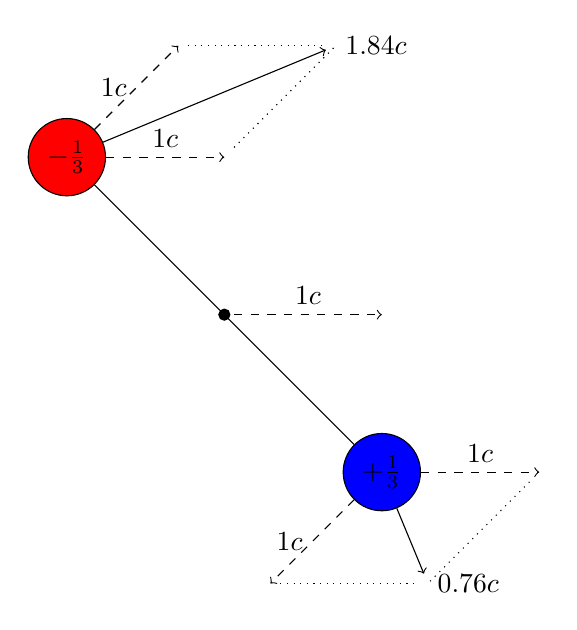
\begin{tikzpicture}[scale=1, rotate=0]


% photon diagonal with speed vectors



\path 
(0,4) node[circle,draw, fill=red](red) {$-\frac{1}{3}$}
(4,0) node[circle,draw, fill=blue](blue) {$+\frac{1}{3}$};
\draw[black] (red) -- (blue)          node[pos=0.5](center){};
\filldraw
 (center) circle (2pt);
\draw[->,dashed, black] (center) -- node[above] { $1c$} ++(2,0) node [anchor=west]{};

%% Arrows indicating the speed components from blue
\draw[->, black, dashed] (blue) -- node[above] { $1c$} ++(2,0) node [](west){};
\draw[->, black, dashed] (blue) -- node[left] { $1c$} ++(225:2) node [](south){};
\draw[ black, dotted] (west) -- ++(225:2) node [](southwest){};
\draw[ black, dotted] (south) -- (southwest) node []{};
\draw[->, black] (blue) --  (southwest) node[below, right] { $0.76c$};

%% Arrows indicating the speed components from red
\draw[->, black, dashed] (red) -- node[above] { $1c$} ++(2,0) node [](redwest){};
\draw[->, black, dashed] (red) -- node[left] { $1c$} ++(45:2) node [](redsouth){};
\draw[ black, dotted] (redwest) -- ++(45:2) node [](redsouthwest){};
\draw[ black, dotted] (redsouth) -- (redsouthwest) node []{};
\draw[->, black] (red) --  (redsouthwest) node[below, right] { $1.84c$};

\end{tikzpicture}


\section{}
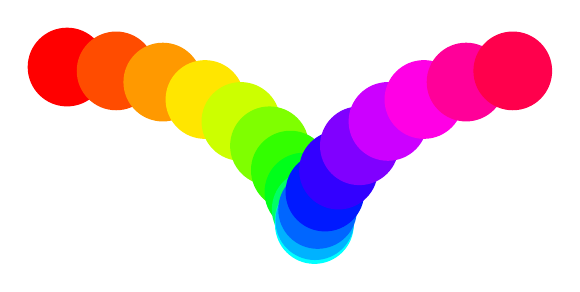
\begin{tikzpicture}[scale=1, rotate=0]

% photon going through cycloid cycle in colors
 \foreach \x in {0, 0.05,...,1}
  {
  \definecolor{reddish}{hsb}{\x, 1, 1}
  \draw[draw=none, fill=reddish] 
   ({((2*pi*\x + sin(2*pi*\x r)) },{1 + cos(2*pi*\x r) }) circle [radius=0.5];

  }

\end{tikzpicture}



\section{}
\begin{tikzpicture}[scale=1, rotate=0]

% single ornac of a photon going through cycloid cycle in colors
 \foreach \x in {0, 0.05,...,1}
  {
  \definecolor{reddish}{hsb}{\x, 1, 1}
  \draw[black, fill=reddish] 
   ({((2*pi*\x + sin(2*pi*\x r)) },{1 + cos(2*pi*\x r) }) circle [radius=0.05];

  }

\end{tikzpicture}



\section{}
\begin{tikzpicture}[scale=1, rotate=0]

% single ornac of a photon  going through two cycloid cycle in red

%% red ornac
 \foreach \x in {0, 0.05,...,2}
  {
  
  \draw[black, fill=red] 
   ({((2*pi*\x + sin(2*pi*\x r)) },{1 + cos(2*pi*\x r) }) circle [radius=0.05];

  }

\path
(3*pi,0) node (bottom){};

\draw[<-, thick] (bottom) -- ++(1,-1) node (slowspeed){}; 
\path
(slowspeed) node [anchor=west, align=right]{slowest speed = $\emptyset$};

\end{tikzpicture}




\section{}
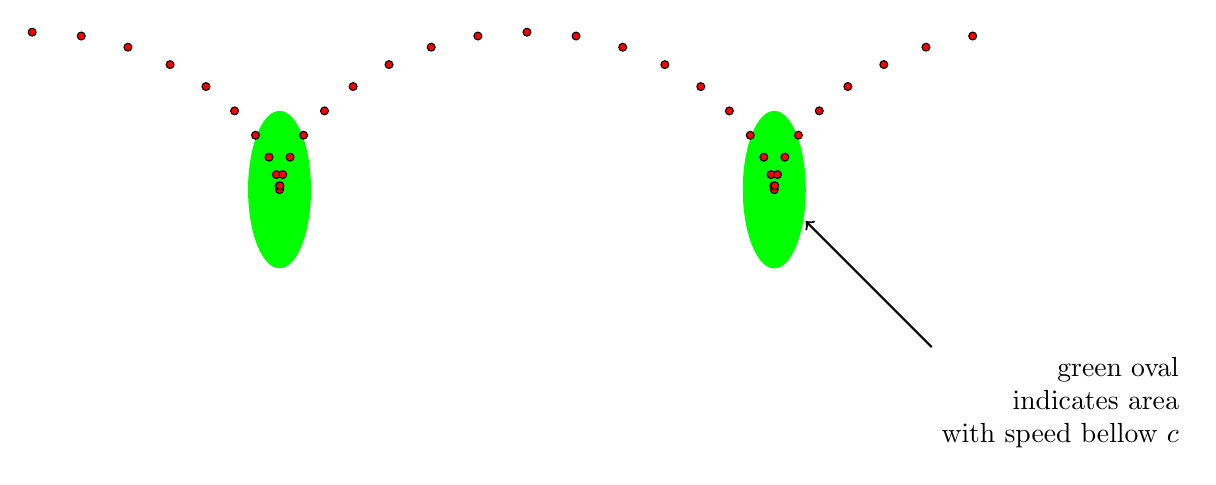
\begin{tikzpicture}[scale=1, rotate=0]

% single ornac of a photon  going through two cycloid cycle in red
% with green oval to indicate the under c area

% greeen oval
\path
(pi,0) node (bottom1){}
(3*pi,0) node (bottom2){};
\draw [draw = none, fill = green]
 (bottom1) circle [ x radius = 0.4, y radius = 1 ]
 (bottom2) circle [ x radius = 0.4, y radius = 1 ]node (greenoval) {};

\draw[<-, thick] (greenoval)+(0.4,-0.4) -- ++(2,-2) node (slowspeed){}; 
\path
(slowspeed) node [below right , align=right]
{green oval \\ indicates area \\ with  speed bellow $c$};


%% red ornac
 \foreach \x in {0, 0.05,...,2}
  {
    \draw[black, fill=red] 
   ({((2*pi*\x + sin(2*pi*\x r)) },{1 + cos(2*pi*\x r) }) circle [radius=0.05];
  }


\end{tikzpicture}



\section{}
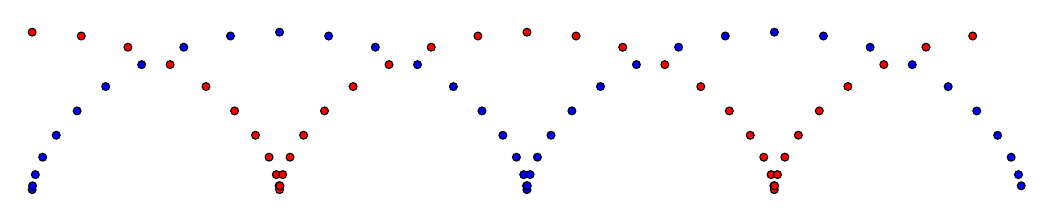
\begin{tikzpicture}[scale=1, rotate=0]

% two ornac of a photon  going through two cycloid cycle in red

%% red ornac
 \foreach \x in {0, 0.05,...,2}
  {
    \draw[black, fill=red] 
   ({((2*pi*\x + sin(2*pi*\x r)) },{1 + cos(2*pi*\x r) }) circle [radius=0.05];
  }


%% blue ornac
 \foreach \x in {0, 0.05,...,2}
  {
    \draw[black, fill=blue] 
   ({((2*pi*\x + sin((2*pi*\x -pi) r)) },{1 + cos((2*pi*\x -pi) r) }) circle [radius=0.05];
  }

\end{tikzpicture}


\section{}
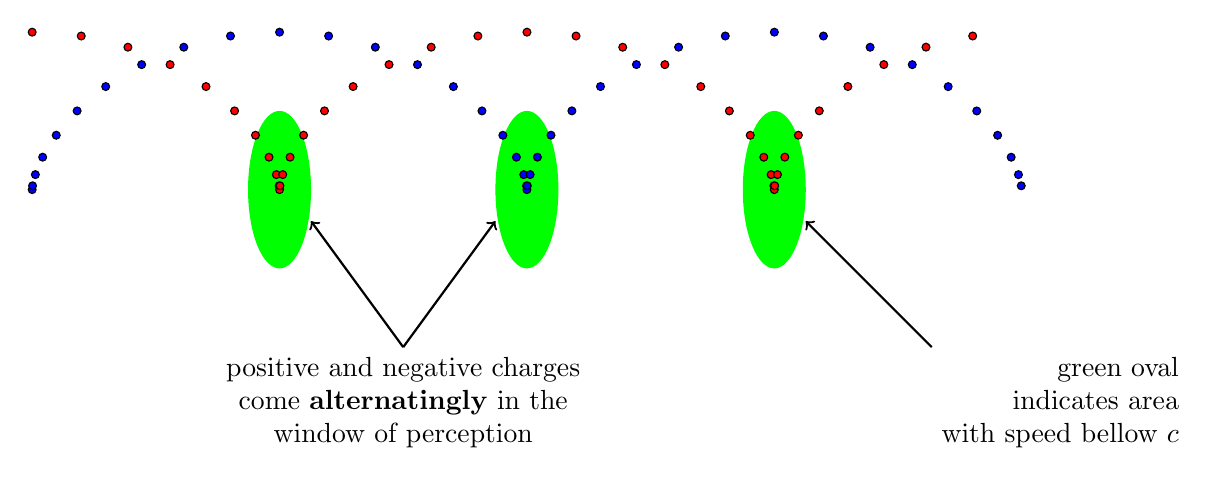
\begin{tikzpicture}[scale=1, rotate=0]

% two ornac of a photon  going through two cycloid cycle in red and blue
% with green oval to indicate the under c area

% greeen ovals
 \foreach \p in {1,...,3}
    \draw [draw = none, fill = green]
     (pi*\p,0) circle [ x radius = 0.4, y radius = 1 ];

\path
(3*pi,0) node (greenoval) {};
\draw[<-, thick] (greenoval)+(0.4,-0.4) -- ++(2,-2) node (slowspeed){}; 
\path
(slowspeed) node [below right , align=right]
{green oval \\ indicates area \\ with  speed bellow $c$};

\path
(1*pi,0) node (greenoval1) {}
(2*pi,0) node (greenoval2) {};
\draw[<-, thick] (greenoval1)+(0.4,-0.4) -- (1.5*pi,-2) node (alternatingly){}; 
\draw[<-, thick] (greenoval2)+(-0.4,-0.4) -- (1.5*pi,-2) node {}; 
\path
(alternatingly) node [below , align=center]
{positive and negative charges \\ come  \textbf{alternatingly} in the \\ window of perception};


%% red ornac
 \foreach \x in {0, 0.05,...,2}
  {
    \draw[black, fill=red] 
   ({((2*pi*\x + sin(2*pi*\x r)) },{1 + cos(2*pi*\x r) }) circle [radius=0.05];
  }


%% blue ornac
 \foreach \x in {0, 0.05,...,2}
  {
    \draw[black, fill=blue] 
   ({((2*pi*\x + sin((2*pi*\x -pi) r)) },{1 + cos((2*pi*\x -pi) r) }) circle [radius=0.05];
  }

\end{tikzpicture}


\end{document}

